% LoVullo Specification Specification
%
% Yep.

\documentclass[draft]{lvspec}
\usepackage{multicol}
\usepackage[final]{graphicx}

\makeatletter
  \def\@lvspec@titlecmd{%
    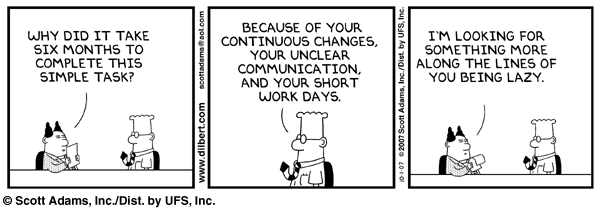
\includegraphics[scale=0.5]{images/dilbert-time.png}
    \vfill
  }%
\makeatother

\begin{document}
\title{LoVullo Specification Specifications}
\author{Mike Gerwitz}
\abstract{%
  \setlength\columnsep{-5ex}%
  \begin{multicols}{2}
  \begin{quote}
    \sl\small\raggedright
    \def\ind{}%
    %
    In the beginning was the plan,\\
    \ind and then the specification;\\
    And the plan was without form,\\
    \ind and the specification was void.

    And darkness\\
    \ind was on the faces of the implementors thereof;\\
    And they spake unto their leader, saying:\\
    ``It is a crock of shit,\\
    \ind and smells as of a sewer.''

    And the leader took pity on them,\\
    \ind and spoke to the project leader:\\
    ``It is a crock of excrement,\\
    \ind and none may abide the odor thereof.''

    And the project leader\\
    \ind spake unto his section head, saying:\\
    ``It is a container of excrement,\\
    \ind and it is very strong, such that none may abide it.''

    The section head then hurried to his department manager,\\
    \ind and informed him thus:\\
    ``It is a vessel of fertilizer,\\
    \ind and none may abide its strength.''
    \goodbreak

    The department manager carried these words\\
    \ind to his general manager,\\
    and spoke unto him\\
    \ind saying:\\
    ``It containeth that which aideth the growth of plants,\\
    \ind and it is very strong.''

    And so it was that the general manager rejoiced\\
    \ind and delivered the good news unto the Vice President.\\
    ``It promoteth growth,\\
    \ind and it is very powerful.''

    The Vice President rushed to the President's side,\\
    \ind and joyously exclaimed:\\
    ``This powerful new software product\\
    \ind will promote the growth of the company!''

    And the President looked upon the product,\\
   \ind and saw that it was very good.

   \hfill---The Jargon File
  \end{quote}
  \end{multicols}
  \bigskip
}
\maketitle

\begindeptgroup{it}

\chapter{Oh, Hello}
\incomplete
\todo{There's no specification yet; in due time.}
\bigskip

\begin{center}
  
\includegraphics[scale=0.5]{images/spec-design.png}
\end{center}


\chapter{Creating Specifications with \LaTeX}
This chapter is an example of an implementation of the specifications and is
useful as an API reference, but \shallnot be used in place of formal
specifications with regards to implementation.

Using the {\tt dwspec} document class with enable paragraph numbering; {\tt
draft} mode will enable signature lines, as shown to the right.

\begin{ex}
  \begin{verbatim}
% omit "[draft]" to disable unapproved signature lines
\documentclass[draft]{lvspec}

% as is the case with all LaTeX documents, begin and end with document
% environment
\begin{document}
  % ...content here...
\end{document}
  \end{verbatim}
\end{ex}

Example environments, as shown above, can be created with the {\tt ex}
environment. All examples end with `$\square$'.

\begin{ex}
  \begin{verbatim}
\begin{ex}
  % ...example here...
\end{ex}
  \end{verbatim}
\end{ex}


\section{Paragraph Numbering}
Paragraph numbering can be temporarily disabled using \verb|\pnumoff| and
re-enabled using \verb|pnumon|\ldots

\pnumoff
\ldots as shown here.

\pnumon
Numbers will continue where they previously left off before being suppressed.

Disabling paragraph numbering also disables the signature line

\begin{ex}
  \begin{verbatim}
Paragraph numbering can be temporarily disabled using \verb|\pnumoff| and
re-enabled using \verb|pnumon|\ldots

\pnumoff
\ldots as shown here.

\pnumon
Numbers will continue where they previously left off before being suppressed.
  \end{verbatim}
\end{ex}


\section{Signature Lines}
The department for the entire section can be set using the
\verb|\sectiondept| command; the command takes effect until the next section
or chapter.

\begin{ex}
  \begin{verbatim}
\section{Signature Lines}
\sectiondept{it}
The department for the entire section can be set using the
\verb|\sectiondept| command; the command takes effect until the next section
or chapter.
  \end{verbatim}
\end{ex}

\dept{pm}
The department can be set per-paragraph using the \verb|\dept| command, as
demonstrated in this paragraph; the command will override any
\verb|\sectiondept| command temporarily and will undo itself after the paragraph
ends.

\begin{ex}
  \begin{verbatim}
\dept{pm}
The department can be set per-paragraph using the \verb|\dept| command, as
demonstrated in this paragraph; the command will override any
\verb|\sectiondept| command temporarily and will undo itself after the paragraph
ends.
  \end{verbatim}
\end{ex}

\dept{it}
An arbitrary group of paragraphs may have their section set using
\verb|\begindeptgroup| and \verb|\enddeptgroup|; they are \emph{not} reset by
sections. They may be nested.

\begin{ex}
  \begin{verbatim}
\begindeptgroup{it}
  % group: it
  \begindeptgroup{pm}
    % group: pm
  \enddeptgroup
  % group: it
\enddeptgroup
  \end{verbatim}
\end{ex}

Clicking on the department in the signature line will take you to the
^[authorization parties] section of the definitions (in this document,
\sref{authorize}).

\subsection{Incomplete}
\incomplete
If a paragraph is incomplete and not yet ready for authorization, use
\verb|\incomplete|.

\begin{ex}
  \begin{verbatim}
\incomplete
If a paragraph is incomplete and not yet ready for authorization, use
\verb|\incomplete|.
  \end{verbatim}
\end{ex}

\incompletei
If a paragraph is incomplete because more information is needed, then use the
command \verb|\incompletei|, which also includes the name of the department.

\begin{ex}
  \begin{verbatim}
\incompletei
If a paragraph is incomplete because more information is needed, then use the
command \verb|\incompletei|, which also includes the name of the department.
  \end{verbatim}
\end{ex}

\enddeptgroup
\end{document}
